\documentclass{beamer}
\usetheme{metropolis} 
\usepackage{listings}
\usepackage{xcolor}
\definecolor{myBlue}{RGB}{0, 0, 180}
\definecolor{myGreen}{RGB}{34, 139, 34}
\definecolor{myRed}{RGB}{180, 0, 0}
\definecolor{myGray}{RGB}{96, 96, 96}
\lstset{ 
    language=Python,
    basicstyle=\ttfamily\tiny,
    keywordstyle=\color{myBlue},
    commentstyle=\color{myGreen},
    stringstyle=\color{myRed},
    showstringspaces=false,
    numberstyle=\tiny\color{myGray},
    stepnumber=1,
    numbersep=5pt,
    frame=single,
    breaklines=true,
    breakatwhitespace=true,
    tabsize=4,
    captionpos=b
}
\title{Chapter 2: Multi-armed Bandits}
\date{\today}
\author{Gabe Sekeres}
\institute{Cornell University}
\begin{document}

  \maketitle
  
\section{$\varepsilon$-Greedy Bandits}
  
\begin{frame}{Introduction}
	\begin{itemize}
		\item We have a simple environment: 10 arms, where each arm $k_i$ is defined by \[k_i \sim \mathcal{N}(q_i,1) \quad \text{ where } q_i \sim \mathcal{N}(0,1), i = 1,\dots,10\]
		\item The text considers three different bandit algorithms: $\varepsilon$-greedy, upper confidence bound (UCB), and gradient
		\item Here, I show only the code for $\varepsilon$-greedy. I did replicate the others in Julia, the full code is in \alert{\href{https://github.com/gsekeres/cornell_theory_reading_group_RL/tree/main/chapter02}{the Github repo}}.
	\end{itemize}
	\emph{Remark.} These are actual reinforcement learners, as opposed to the Tic-tac-toe players, which functioned more as supervised learners than anything. I'm unsure why that was the first example, as this is significantly more intuitive (and easier to code).
\end{frame}
  
 \begin{frame}{Reward Distributions (fig. 2.1)}
 	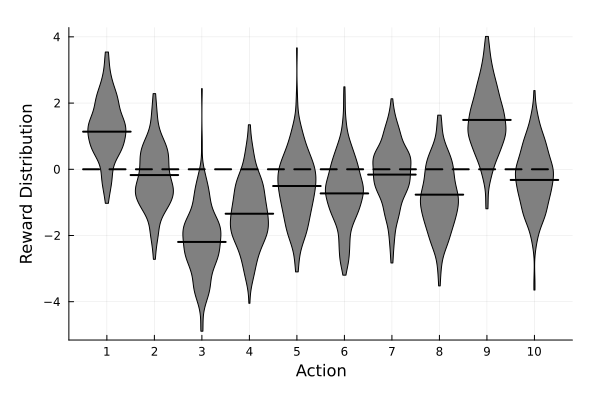
\includegraphics[width=11cm]{ten_armed_testbed_violin.png}
 \end{frame}
 
 \begin{frame}{Bandit Class}
 	As before, we initialize the bandits as a class that is essentially a tuple. I'm ignoring everything irrelevant for the $\varepsilon$-greedy bandits, which simplifies things a lot. We have: 
 	\[
 	\text{Bandit} = \langle k, \alpha, \varepsilon, q_0, \{q_i\},\mathbb{E}\{q_i\}, \{\text{actions}\}, \text{bestAction}\rangle 
 	\]
 	Everything that follows runs through the bandit class. The other types of learners are initialized by adding more parameters to the class and if-statements to the functions.
 \end{frame}
 
\begin{frame}[fragile]{Bandit Functions - reset(Bandit)}
\begin{itemize}
	\item Sets the true rewards, the initial estimations, and resets the actions, best action, and number of actions taken.
\end{itemize}
\begin{lstlisting}
def reset(self):
    # real reward for each action
    self.q_true = np.random.randn(self.k) + self.true_reward

    # estimation for each action
    self.q_estimation = np.zeros(self.k) + self.initial

    # # of chosen times for each action
    self.action_count = np.zeros(self.k)

    self.best_action = np.argmax(self.q_true)

    self.time = 0
\end{lstlisting}
\end{frame}
\begin{frame}[fragile]{Bandit Functions - act(Bandit) $\to$ action}
\begin{itemize}
	\item Take an action -- random if \texttt{rand()} $\sim \text{Uniform}[0,1)$ less than $\varepsilon$, greedy otherwise.
\end{itemize}
\begin{lstlisting}
def act(self):
    if np.random.rand() < self.epsilon:
        return np.random.choice(self.indices)

    q_best = np.max(self.q_estimation)
    return np.random.choice(np.where(self.q_estimation == q_best)[0])
\end{lstlisting}
\end{frame}
\begin{frame}[fragile]{Bandit Functions - step(Bandit, action) $\to$ reward}
\begin{itemize}
	\item Take an action, and update the estimation for that action
\end{itemize}
\begin{lstlisting}
def step(self, action):
    # generate the reward under N(real reward, 1)
    reward = np.random.randn() + self.q_true[action]
    self.time += 1
    self.action_count[action] += 1
    self.average_reward += (reward - self.average_reward) / self.time

    if self.sample_averages: #always true for this case
        # update estimation using sample averages
        self.q_estimation[action] += (reward - self.q_estimation[action]) / self.action_count[action]
    else:
        # update estimation with constant step size
        self.q_estimation[action] += self.step_size * (reward - self.q_estimation[action])
    return reward
\end{lstlisting}
\end{frame}
\begin{frame}[fragile]{simulate(runs, time, bandits) $\to$ (best\_actions, rewards)}
\begin{itemize}
	\item Simulate some number of runs of length time for some set of bandits, and return the (i) mean rewards and (ii) percent of time the best action was taken
\end{itemize}
\begin{lstlisting}
def simulate(runs, time, bandits):
    rewards = np.zeros((len(bandits), runs, time))
    best_action_counts = np.zeros(rewards.shape)
    for i, bandit in enumerate(bandits):
        for r in trange(runs): #tqdm(range(runs)), tracks progress
            bandit.reset()
            for t in range(time):
                action = bandit.act()
                reward = bandit.step(action)
                rewards[i, r, t] = reward
                if action == bandit.best_action:
                    best_action_counts[i, r, t] = 1
    mean_best_action_counts = best_action_counts.mean(axis=1)
    mean_rewards = rewards.mean(axis=1)
    return mean_best_action_counts, mean_rewards
\end{lstlisting}
\end{frame}
\begin{frame}[fragile]{Rest of Code}
\begin{itemize}
	\item Now all we have to do is set the $\varepsilon$ levels, initialize the bandits, and simulate!
\end{itemize}
\begin{lstlisting}
runs = 2000
time = 1000
epsilons = [0, 0.1, 0.01]
bandits = [Bandit(epsilon=eps, sample_averages=True) for eps in epsilons]
best_action_counts, rewards = simulate(runs, time, bandits)
\end{lstlisting}
\end{frame}
  
  \begin{frame}{Epsilon Reward Comparison (fig. 2.2a)}
  	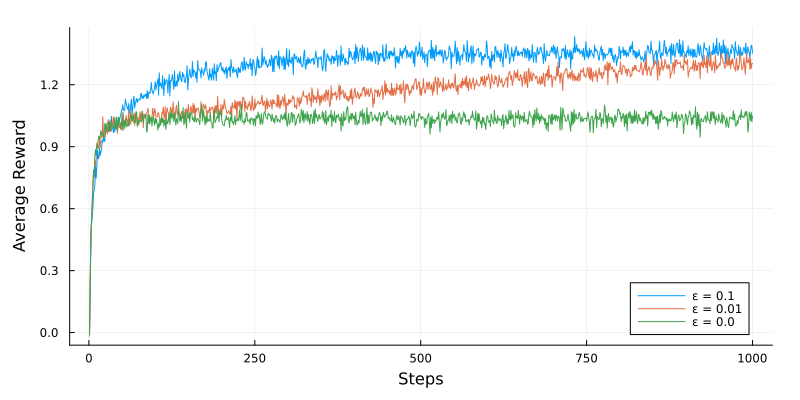
\includegraphics[width=11cm]{ten_armed_testbed_epsilon_greedy.png}
  \end{frame}
  
    \begin{frame}{Epsilon Action Comparison (fig. 2.2b)}
  	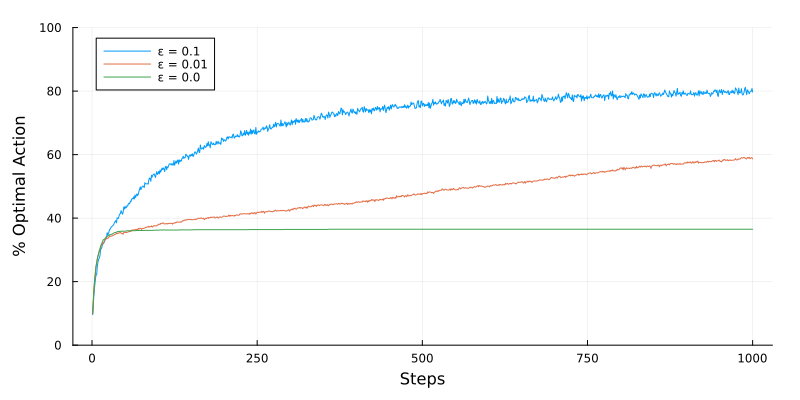
\includegraphics[width=11cm]{ten_armed_testbed_epsilon_optimal.png}
  \end{frame}
  
  \section{Other Bandit Replications}
  
\begin{frame}{Optimistic vs. Realistic (fig. 2.3)}
	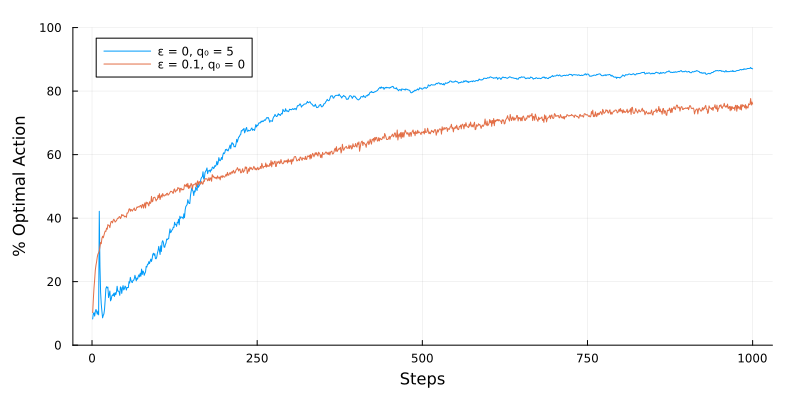
\includegraphics[width=11cm]{ten_armed_testbed_optimistic.png}
\end{frame}
\begin{frame}{UCB vs. Epsilon (fig. 2.4)}
	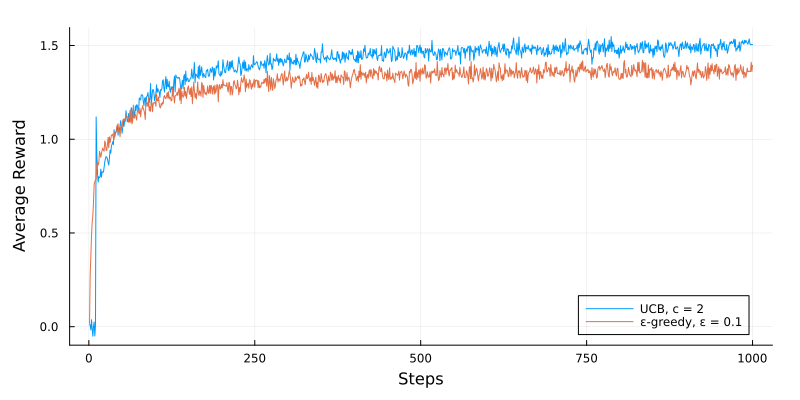
\includegraphics[width=11cm]{ten_armed_testbed_ucb.png}
\end{frame}
\begin{frame}{Gradient Baseline Comparison (fig. 2.5)}
	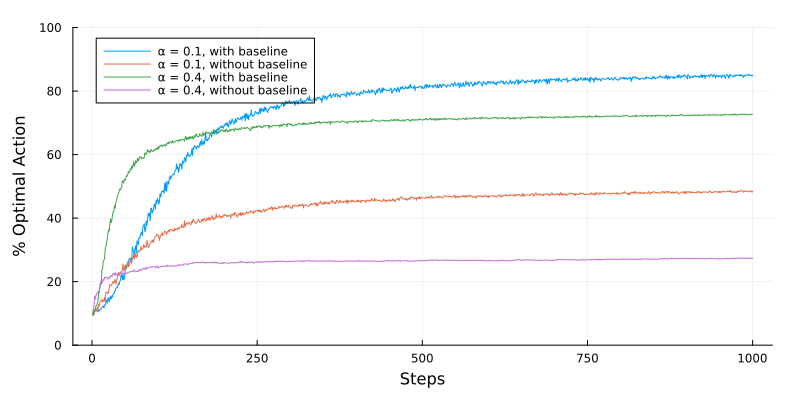
\includegraphics[width=11cm]{ten_armed_testbed_gradient.png}
\end{frame}
\begin{frame}{Full Bandit Comparison (fig. 2.6)}
	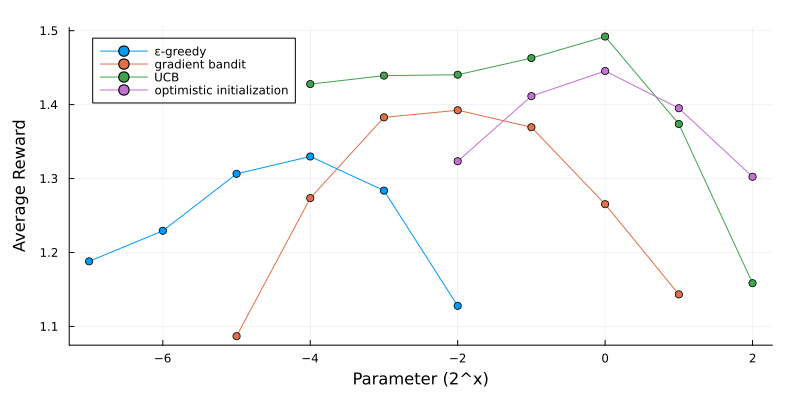
\includegraphics[width=11cm]{ten_armed_testbed_comparison.png}
\end{frame}
  
  
  
\end{document}